\begin{figure}
    \centering
    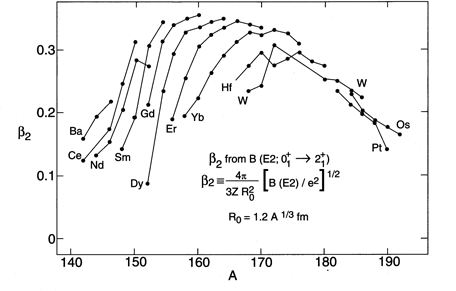
\includegraphics[scale=2]{Introduction_Figs/DeformationParamCasten.png}
    \caption{Plot of the deformation parameter $\beta_2$ along isotopic chains. Deformation can be seen setting in, as isotopic chains transition from spherical to deformed. The formula to calculate $\beta_2$ from the reduced transition probability is shown. This $\beta_2$, is an absolute measure of deformation, and does not distinguish between prolate and oblate. Taken from \citep{casten90:_structure}.}
    \label{fig:beta_by_isotope}
\end{figure}